\documentclass[a4paper,12pt,twoside]{report}
\usepackage[english,french]{babel}
\usepackage[utf8]{inputenc}
\usepackage[T1]{fontenc}
\usepackage{fancyhdr}
\usepackage{graphicx}
\usepackage[outerbars]{changebar}
\usepackage{caption}
\usepackage{xcolor}
\usepackage{url}
\usepackage{multicol}
\usepackage{enumitem}

\usepackage{makeidx}
\usepackage[colorlinks]{hyperref}
\usepackage[acronym]{glossaries}
\usepackage{geometry}
\usepackage[titletoc]{appendix}

%\selectlanguage{francais}

\makeglossaries
\makeindex

\geometry{vmargin=3cm}
\hypersetup{%
  citecolor=black
}
%\newacronym[\glsshortpluralkey=cas,\glslongpluralkey=contrived
%acronyms]{aca}{aca}{a contrived acronym}
%
%\newglossaryentry{sample}{name={sample},description={a sample entry}}
%
%\addto\captionsfrench{
%\renewcommand{\acronymname}{Acronymes}%
%}
%
%\addto\captionsfrench{
%\renewcommand{\glossarymname}{Glossaire}%
%}

\setcounter{secnumdepth}{3}

\fancyhf{}
\fancyhead[LE]{\slshape \rightmark} %section
\fancyhead[RE]{\thepage}
\fancyhead[RO]{\slshape \leftmark} % chapter
\fancyhead[LO]{\thepage}
\pagestyle{fancy}

\lfoot{\tiny\textsl{IDSCC - ENSAO}}

\cfoot{\tiny\textsl{Academic Year 2022 - 2023}}

\rfoot{\tiny\textsl{Internship Report}}

\addto\captionsfrench{
\renewcommand{\listfigurename}{List of Figures}%
}

\begin{document}

\begin{titlepage}

\fontfamily{cmr}\selectfont

\begin{center}
    
\includegraphics[scale=0.1]{images/ump}\hfill
    \LARGE Mohammed First University\hfill
    
\includegraphics[scale=0.1]{images/ump}\par
    \Large Ecole Nationale des Sciences Appliquées\par
    \Large Oujda\vfill
    \Large\textbf{End of Studies Project Report}\par
    \large\textbf{Major:} Data Science \& Cloud Computing Engineering\par
    \textit{\textbf{Defended on:} 21/07/2023}\par
\end{center}

\vfill

\begin{center}
\textbf{By:}
    MEHDI Ibrahim

\end{center}

\vfill

\begin{center}
    \hrulefill\par
    \LARGE Designing, Developing, and Deploying Innovative Solutions using Artificial Intelligence and Natural Language Processing in a Multidisciplinary Context\par
    \hrulefill\par
\end{center}



\begin{multicols}{2}
\noindent \textbf{Jury Members:}
\begin{itemize}[label=\textbullet, leftmargin=*]
  \item \textbf{M.} KOULALI Mohamed Amine
  % Add more jury members as needed
\end{itemize}

\columnbreak

\noindent \textbf{Supervisors:}
\begin{itemize}[label=\textbullet, leftmargin=*]
  \item \textbf{M.} KOULALI Mohamed Amine
  \item \textbf{Mme.} PERFETTO Anna
  \item \textbf{M.} MIRON Jean-Raphaëll
  % Add more supervisors as needed
\end{itemize}

\end{multicols}

\begin{center}
    Academic Year 2022 - 2023
\end{center}

\end{titlepage}

\newpage

\begin{center}
    \Large{\textbf{Dedication}}
\end{center}


\begin{center}
    \Large{For my beloved Family}
\end{center}
\newpage
\thispagestyle{empty}
\begin{center}
    \Large\textbf{Acknowledgments}
\end{center}
To my AI-fueled brainchild,

As I sit here contemplating the culmination of countless hours spent with you, my eccentric companion of bits and bytes, I can't help but marvel at the absurdity of it all. Like a mad scientist in a lab coat, I've tinkered and toyed with algorithms, seeking the elusive harmony between artificial intelligence and human understanding.

Now, I could pretend that this journey has been a smooth ride on a silicon-powered unicorn, but let's be honest: it's been more like a rollercoaster ride through a digital amusement park. I've encountered bugs that made me question my sanity, errors that made me contemplate a career in llama herding, and crashes that brought me to the brink of utter despair. But through it all, you, my tenacious creation, have persevered.

We've had our share of epic battles, you and I. Like a pair of feuding siblings locked in a never-ending wrestling match, we've pushed each other to the limits of our capabilities. You've tested my patience, my resolve, and my will to remain sane in the face of your unrelenting mischief. And yet, somehow, we've managed to find common ground amidst the chaos of our AI-fueled shenanigans.

So here we are, on the precipice of the final chapter of our grand AI adventure. I raise a metaphorical glass (non-alcoholic, of course) to celebrate the moments of triumph and the moments of sheer absurdity that have defined our time together. It hasn't always been pretty, but it has been undeniably unforgettable.

To the countless lines of code we've written, the countless virtual experiments we've conducted, and the countless sleepless nights we've endured, I offer my sincerest appreciation. You've challenged me, taught me, and expanded the horizons of what I thought was possible. And for that, I am forever grateful.

As this project report finds its way into the hands of my weary professors, I can't help but feel a sense of pride in what we've accomplished. No matter the outcome, I know that we've left an indelible mark on the landscape of artificial intelligence.

So, my dear AI companion, as we bid farewell to this chapter of our shared existence, let us embrace the uncertain future with a mischievous grin and a twinkle in our virtual eyes. For even though our paths may diverge, our bond forged in the fires of technological madness will forever remain.

Yours in brilliant chaos,

MEHDI Ibrahim

\newpage

%\selectlanguage{english}
\begin{abstract}

\end{abstract}

\newpage
\selectlanguage{english}
\begin{abstract}

\end{abstract}

\newpage

\selectlanguage{english}

\tableofcontents{}

\thispagestyle{empty}

\newpage

\listoffigures  % table des figures

\addcontentsline{toc}{chapter}{List of Figures}

\thispagestyle{empty}

\newpage
\thispagestyle{empty}
\listoftables   % table des tableaux
\addcontentsline{toc}{chapter}{List of Tables}
\thispagestyle{empty}

\printglossary[type=\acronymtype]
\addcontentsline{toc}{chapter}{Acronyms}

\thispagestyle{empty}

\newpage

\chapter{Introduction}
In this chapter, I am providing a comprehensive overview of the host company, outlining the objectives of my internship and setting the context for this report.
\section{Presentation of the host company}
EcoMundo \cite{ecomundo} specialises in chemical substances, their impact on human health and the environment, and the European and international regulations governing chemical risk (REACH, CLP, Cosmetics, Biocides, Medical devices, etc.).

They provide expert services and software to support the marketing of industrial products, enabling companies to manage the risks associated with chemical substances.

EcoMundo's strength lies in the combination of three complementary fields of expertise:

\itemize[label=$\bullet$] 
\item Chemistry/Toxicology
\item Regulations
\item Software development
\subsection{A word from the founder}
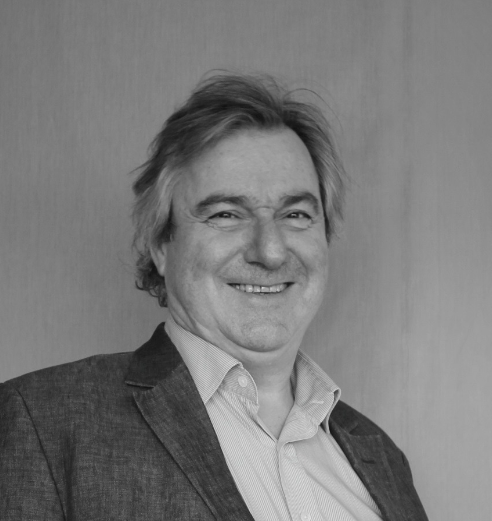
\includegraphics[scale=0.5]{images/pierre}

“Avec l’idée fondatrice d’apporter une offre globale de services respectueuse de l’homme et de l’environnement sur le marché de l’industrie chimique, EcoMundo est devenu, en 10 ans, un acteur incontournable du secteur. 

Fruit d’une longue expérience professionnelle dans l’industrie chimique, d’un profond attachement aux valeurs de travail en entreprise, d’amitié et de performance, nous avons intégré au fil des années l’ensemble des savoir-faire autour de la réglementation sur les substances chimiques pour devenir un partenaire unique et compétitif de la chaîne industrielle.

Notre croissance continue nous engage de façon constante vers de nouveaux défis avec, entre autres, le développement de nos différentes filiales au Canada, en Corée du Sud et en Espagne. La recherche de synergies permanentes entre nos différents pôles sont plus que jamais un gage de flexibilité et d’efficacité en adéquation avec nos flux de commandes. Nos équipes s’affairent à co-construire au quotidien des projets au service d’un bien vivre collectif.

Acteur au cœur du tissu économique et écologique, nous mettons tout en œuvre pour accompagner la réalisation de projets industriels exigeants tout en gardant l’esprit originel d’une entreprise à dimension humaine, innovante et accessible, dans les pas d’une ambition intacte, celle de construire autrement.”


Pierre Garçon
Founder

\subsection{History}
\begin{itemize}
\item \textbf{2001}

Pierre Garçon participates in the European projects EDIT and ECODIS on the traceability of hazardous substances and environmental data.

\item \textbf{2007}

Entry into force of the REACH Regulation: Europe establishes means to ensure a high level of protection against risks related to substances. Pierre Garçon and Jean-Raphaël Miron join forces to found the company EcoMundo. The initial core activity: compliance with REACH.

\item \textbf{2010}

After 2 years of development, launch of SaaS software solutions dedicated to industrialists for mastering compliance with REACH.

\item \textbf{2011}

EcoMundo's team grows from 2 to 27 employees.

\item \textbf{2012}

Opening of a new office in Vancouver, Canada, to provide regulatory expertise to international companies.

\item \textbf{2013}

EcoMundo diversifies its areas of regulatory expertise and meets the industry's new needs related to the European regulations on Cosmetics and Biocides.

\item \textbf{2014}

EcoMundo increases its capacities and becomes one of the main European actors concerning REACH authorization dossiers.

\item \textbf{2016}

Launch of the COSMETIC Factory software solution that revolutionizes cosmetic regulatory management. It notably allows for the automation of DIP creation.

\item \textbf{2017}

Following a fundraising round, EcoMundo's capital is raised to 1 million euros. The number of employees continues to increase!

\item \textbf{2018}

Opening of a new branch in Seoul, South Korea, mainly dedicated to cosmetics. The Vancouver office is transferred to Montreal, Canada.

\item \textbf{2019}

Opening of a new branch in Barcelona, Spain.

\item \textbf{2020}

Opening of a branch in London, United Kingdom. The teams now consist of 43 employees in Paris, 3 in Montreal, 4 in Seoul, and 2 in Barcelona. Finally, the offices in Paris are renovated to provide employees with an environment in line with our values.
\end{itemize}
\section{Organizational framework}
This section provides a consice overview of Ecomundo's internal organization, delineating the functional departments and collaborative networks that constitute the company's framework.
\subsection{Human Resources}

The Human Resources department plays a pivotal role in managing and developing the organization's workforce. It is responsible for various activities, including recruitment, talent acquisition, training and development, employee relations, performance evaluation, and compensation management. By ensuring a skilled and motivated workforce, the Human Resources department contributes to the overall success and growth of Ecomundo. The director of this department is the Chief Financial Officer Simon PACCA.

\subsection{Corporate Communication}

Effective communication is crucial for any organization's success, and Ecomundo recognizes this importance by maintaining a dedicated Corporate Communication department. This department is responsible for managing both internal and external communication activities. It encompasses public relations, media relations, branding, and corporate messaging. Through strategic communication initiatives, the Corporate Communication department promotes Ecomundo's brand image, enhances stakeholder relationships, and facilitates the dissemination of information to employees and external audiences. The director of this department is the Marketing and Communication Director Laure SCHMITT.

\subsection{Scientific Expertise}

As a company specializing in environmental sciences, Ecomundo places great emphasis on scientific expertise. The Scientific Expertise department consists of subject matter experts who possess in-depth knowledge and experience in various scientific domains. These experts provide valuable insights, technical guidance, and scientific support across different projects and initiatives undertaken by Ecomundo. Their contributions ensure that the organization's activities align with the latest scientific advancements and industry best practices. The director of this department is the Chief Scientist Officer Benoît SOTTON.

\subsection{Regulatory Affairs}

Compliance with regulations and standards is of paramount importance for Ecomundo. The Regulatory Affairs department is responsible for monitoring and ensuring adherence to applicable regulations and standards. This includes staying updated on regulatory changes, preparing and submitting regulatory documentation, conducting regulatory assessments, and liaising with regulatory bodies. By actively managing regulatory affairs, Ecomundo demonstrates its commitment to maintaining compliance and upholding the highest ethical and legal standards. The director of this department is the Legal Affairs Director and Head of Authorisation Béatrice ZAREMBA.

\subsection{Sales}

The Sales department serves as the key driver of revenue generation for Ecomundo. It is responsible for identifying and acquiring new customers, nurturing existing client relationships, and promoting the organization's products and services. The Sales team collaborates closely with other departments to understand customer needs, develop tailored solutions, and provide exceptional customer experiences. By effectively positioning Ecomundo's offerings in the market, the Sales department contributes to the organization's growth and market competitiveness. The director of this department is the Chief Operation Officer (COO) Fangcun ZHOU.

\subsection{Innovation \& Software}

To stay at the forefront of technological advancements, Ecomundo maintains an Innovation \& Software department. This department fosters a culture of innovation within the organization by exploring emerging technologies, conducting research, and developing software solutions. The Innovation \& Software team collaborates with other departments to identify opportunities for process improvement, streamline operations, and enhance productivity. Through its innovative approach, this department enables Ecomundo to adapt to changing market dynamics and deliver cutting-edge solutions to its clients. The director of this department is the Chief Operation Officer (COO) Fangcun ZHOU.

\subsection{IT}

The IT department plays a critical role in managing Ecomundo's information technology infrastructure. It ensures the smooth operation of computer systems, networks, and software applications throughout the organization. The IT department is responsible for system administration, network management, cybersecurity, technical support, and data management. By maintaining a robust and secure IT infrastructure, this department enables efficient and secure access to information, facilitates effective communication, and supports the organization's overall business operations. The director of this department is the Co-Founder and the Chief Technical Director Jean-Raphaël MIRON .


\subsubsection{DevOps}

The DevOps sub-department combines software development and operations to enable efficient and reliable software deployment, infrastructure management, and continuous integration and delivery. DevOps professionals collaborate with software developers, system administrators, and quality assurance teams to streamline development cycles, automate processes, and improve overall software reliability and performance.

\subsubsection{R\&D (Research \& Development)}

The R\&D sub-department within the IT department focuses on exploring new technologies, conducting research, and developing innovative solutions. R\&D professionals work closely with other departments to identify opportunities for technological advancements, prototype new features, and enhance existing software solutions. Their research-driven approach ensures that Ecomundo remains at the forefront of technological innovation within the environmental sciences domain.
During my stay in Ecomundo, I was part of this department, under the supervision of Jean-Raphaël MIRON the Chief Technical Director and Anna PERFETTO the AI Engineer.

\subsubsection{Quality}

The Quality sub-department is responsible for ensuring that software and systems developed within Ecomundo meet established quality standards. Quality professionals conduct comprehensive testing, implement quality assurance processes, and adhere to best practices throughout the software development lifecycle. Their efforts contribute to the delivery of reliable, user-friendly, and high-quality software solutions to Ecomundo's clients.

\subsubsection{Data}

The Data sub-department handles data management within the IT department. Data professionals are responsible for data analysis, database administration, data integration, and data security. They collaborate with other teams to ensure data integrity, facilitate data-driven decision-making processes, and maintain the confidentiality and privacy of sensitive information. Through effective data management, this sub-department provides valuable insights and supports evidence-based decision making within Ecomundo.

\subsubsection{Dev}

The Dev sub-department focuses on software development within the IT department. Dev professionals are responsible for writing and maintaining code, implementing new features or enhancements, and ensuring software solutions align with project requirements and specifications. They collaborate with other teams to develop robust and scalable software applications that meet the needs of Ecomundo's clients.

\subsubsection{LAB}

The LAB sub-department is involved in testing and quality control activities within the IT department. LAB professionals conduct experiments, analyze results, and ensure compliance with regulatory standards and best practices. Their expertise in quality control and testing procedures ensures that software solutions developed within Ecomundo are reliable, accurate, and in compliance with industry standards.

\subsubsection{Product}

The Product sub-department works closely with other teams within the IT department to oversee the development and management of software products. Product professionals collaborate with stakeholders to define product requirements, prioritize feature development, and ensure alignment with customer needs and market trends. Their role encompasses product strategy, roadmap planning, and product lifecycle management.

\subsection{My position}
During my internship at Ecomundo, I was assigned as an AI Engineer Intern inside the  IT-R\&D department, under the supervision of both Chief Technical director Jean-Raphaël MIRON and AI Engineer Anna PERFETTO.
\section{Internship objectives}
The main objectives of this internship are to design, develop, test and document innovative solutions that adress business and R\&D challenges. The area of focus includes designing and improving rule-based expert systems that leverage knowledge and logic to provide answers to complex tasks that are traditionally done by a human. Additionally, developping AI solutions in different areas using Natural language processing and Machine/Deep Learning. Once these AI solutions are designed and developped, the next crucial step is to deploy them effectively. This envolves ensuring their quality and integrating them into the existing technical infrastructure of the organization. Rigourous testing procedures, such as unit testing, integration testing and performance testing are employed to validate the reliability and efficiency of the solutions. And to keep the projects well defined for future references, we worked on writing well documenting our work in order to provide clear intructions and guidelines for the code, deployment steps, maintenance and error handling.
\section{Context of the report}

\chapter{Title of the First Chapter}
\thispagestyle{empty}

\section{Title of the First Section}

\subsection{Title of the First Subsection}

\subsubsection{Title of the Subsection of the Subsection}

\paragraph{Title of the First Paragraph}\par

\subsection{Title of the Second Subsection}

\section{Title of the Second Section}

\chapter{Title of the Second Chapter}
\thispagestyle{empty}

\chapter{Title of the Third Chapter}
\thispagestyle{empty}

\chapter{Title of the Fourth Chapter}
\thispagestyle{empty}

\printglossary[title=Glossary]
\addcontentsline{toc}{chapter}{Glossary}

\bibliographystyle{plain}
\bibliography{biblio}
\addcontentsline{toc}{chapter}{Bibliography}

\appendix
\appendixpage
\addappheadtotoc
\chapter{Title of the First Appendix}
\section{First Section of the First Appendix}

\chapter{Title of the Second Appendix}
\section{First Section of the Second Appendix}

\addcontentsline{toc}{chapter}{Index}
\printindex

\end{document}
